\documentclass[11pt]{article}

\usepackage[a4paper,margin=1in]{geometry}
\usepackage{booktabs}
\usepackage{graphicx}
\usepackage{amsmath}
\usepackage{hyperref}
\usepackage{xcolor}
\usepackage{multirow}
\usepackage{array}
\usepackage{caption}
\usepackage{tabularx}

\definecolor{bestred}{HTML}{C62828}
\definecolor{secondblue}{HTML}{1565C0}
\definecolor{gaingreen}{HTML}{2E7D32}
\newcommand{\best}[1]{\textcolor{bestred}{\textbf{#1}}}
\newcommand{\second}[1]{\textcolor{secondblue}{\underline{#1}}}
\newcommand{\gain}[1]{\textcolor{gaingreen}{#1}}

\title{A DoLPHiN-Derived Polysaccharide Knowledge Graph for Interpretable Function Retrieval and Tail-Sensitive Ontology Propagation}
\author{First Author$^{1}$, Second Author$^{2}$, Corresponding Author$^{1,*}$\\
\small $^{1}$Affiliation 1, City, Country\\
\small $^{2}$Affiliation 2, City, Country\\
\small $^{*}$Correspondence: corresponding.author@email.example}
\date{}

\begin{document}
\maketitle

\begin{abstract}
Polysaccharide bioactivity evidence is scattered across source organisms, monomer composition, linkage patterns, functional annotations, disease associations, and literature provenance, but these signals are rarely organized into graph-native resources that support controlled retrieval benchmarks. We convert DoLPHiN into a heterogeneous polysaccharide knowledge graph with 5,078 polysaccharide nodes linked to organism, monosaccharide, glycosidic bond, function, disease, and publication entities, and use it to study masked \texttt{poly-function} retrieval as the primary benchmark together with a clean unified-split function-prediction diagnostic. The main finding is not that a new graph model dominates all baselines, but that the current KG already supports useful interpretable retrieval. Under the leakage-controlled clean diagnostic setting, the strongest benchmark is a regularized shallow classifier on explicit meta-path features, reaching test macro-F1 0.3465; adding the corrected disease-free \texttt{poly\_x} block gives 0.3317. The current hetero GNN, no-message ablation, and node-local MLP remain much weaker at 0.0464, 0.0426, and 0.0466. Failure ablations show that removing message passing leaves the GNN almost unchanged, indicating that the immediate bottleneck is graph representation rather than optimizer tuning. Disease-aware retrieval serves as an upper-bound semantic setting rather than the main clean claim. In that upper-bound regime, confidence-gated parent/child ontology propagation provides a selective, mechanism-level tail intervention without changing the global ranking profile in a practically meaningful way: across 16 paired seeds and 16,000 masked edges, tail micro filtered Hits@3 improves from 0.0552 to 0.1021, with one-sided paired McNemar p = 0.03125 and tail filtered MRR gain 0.0395 with permutation p = 0.0002499. These results position the DoLPHiN-derived KG as a useful substrate for interpretable polysaccharide function retrieval and show that ontology is most helpful here as selective parent/child evidence routing rather than as coarse family smoothing.
\end{abstract}

\noindent\textbf{Database URL:} \texttt{[INSERT-DATABASE-URL]}. The public landing page should provide open access to the DoLPHiN-derived knowledge graph, benchmark data, and documentation.

\section{Introduction}
\label{sec:introduction}

Long-chain polysaccharides occupy a difficult but important space in biomolecular research because their biological roles emerge from heterogeneous structural cues, source-dependent context, and sparse functional evidence. Unlike many small-molecule or protein prediction settings, polysaccharide studies are fragmented across domain-specific databases and literature records, and their evidence is often stored as semi-structured text rather than machine-actionable graphs. This fragmentation limits not only downstream prediction, but also mechanistic querying, provenance tracking, and hypothesis generation.

DoLPHiN is a useful starting point because it aggregates polysaccharide-centered records that already expose several relevant evidence channels, including source organisms, monomer composition, linkage patterns, functional labels, disease associations, and DOIs~\cite{xin2025dolphin}. Yet the raw records are not immediately suitable for graph learning or structured retrieval. Important entities still appear as free text, heterogeneous relations are not explicitly typed, and provenance is not arranged in a way that supports transparent graph-native evaluation.

This paper addresses that gap by transforming DoLPHiN into a heterogeneous polysaccharide knowledge graph and then using this graph to study masked \texttt{poly-function} retrieval as the primary benchmark. We additionally use a unified-split multi-label function-prediction task as a clean diagnostic benchmark for measuring how much signal is recoverable from explicit typed graph evidence before ontology or disease-aware semantics are introduced. Our goal is deliberately narrower than proposing a universally superior predictor. Instead, we focus on three questions that are useful for both resource building and method design. First, can a DoLPHiN-derived KG provide usable supervision for polysaccharide function retrieval at all? Second, on the current graph version, are the strongest clean signals better captured by interpretable relation-derived feature models or by hetero GNN message passing? Third, can ontology support improve the rare-label regime without materially distorting the stronger disease-aware upper bound? Figure~\ref{fig:pipeline} summarizes the resulting data-to-graph-to-retrieval workflow.

Our empirical answers are specific. The KG is already useful, but its strongest clean signal is currently exposed through explicit shallow feature models rather than through end-to-end message passing. On a unified train/valid/test split, a regularized one-vs-rest logistic model on leakage-controlled meta-path incidence features reaches test macro-F1 0.3465, while adding the corrected disease-free \texttt{poly\_x} block gives 0.3317. In contrast, the current hetero GNN, no-message ablation, and node-local MLP remain near 0.04--0.05 macro-F1. Failure ablations show that removing message passing leaves these GNNs almost unchanged, which suggests that the immediate bottleneck is not simply missing tuning but a mismatch between the present graph representation and what shallow neighborhood aggregation can exploit. Disease-aware variants are substantially stronger, but they are interpreted here as upper-bound side information because disease nodes are tightly coupled to the target functions. Figure~\ref{fig:benchmarks} gives the narrative benchmark summary, while Tables~\ref{tab:clean-diagnostic},~\ref{tab:retrieval-results}, and~\ref{tab:gnn-ablation} provide the exact corresponding values.

The final part of the paper focuses on the long tail. Many ontology formulations we tried either acted as near no-ops or degraded ranking by oversmoothing function families. The useful variant emerged only after converting ontology support into confidence-gated parent/child propagation that selectively reinforces low-support function candidates during retrieval. This mechanism does not create a new overall best model; instead, it preserves the disease-aware upper bound while providing a stable tail-sensitive gain. We therefore present the ontology result as a task-specific mechanism study rather than as a broadly validated ontology-learning method. The main contribution of the paper is a bounded one: a DoLPHiN-derived KG benchmark that clarifies what currently works on this resource, what currently fails, and where ontology becomes useful only as selective graph-native evidence for tail-sensitive retrieval.

\begin{figure*}[t]
\centering
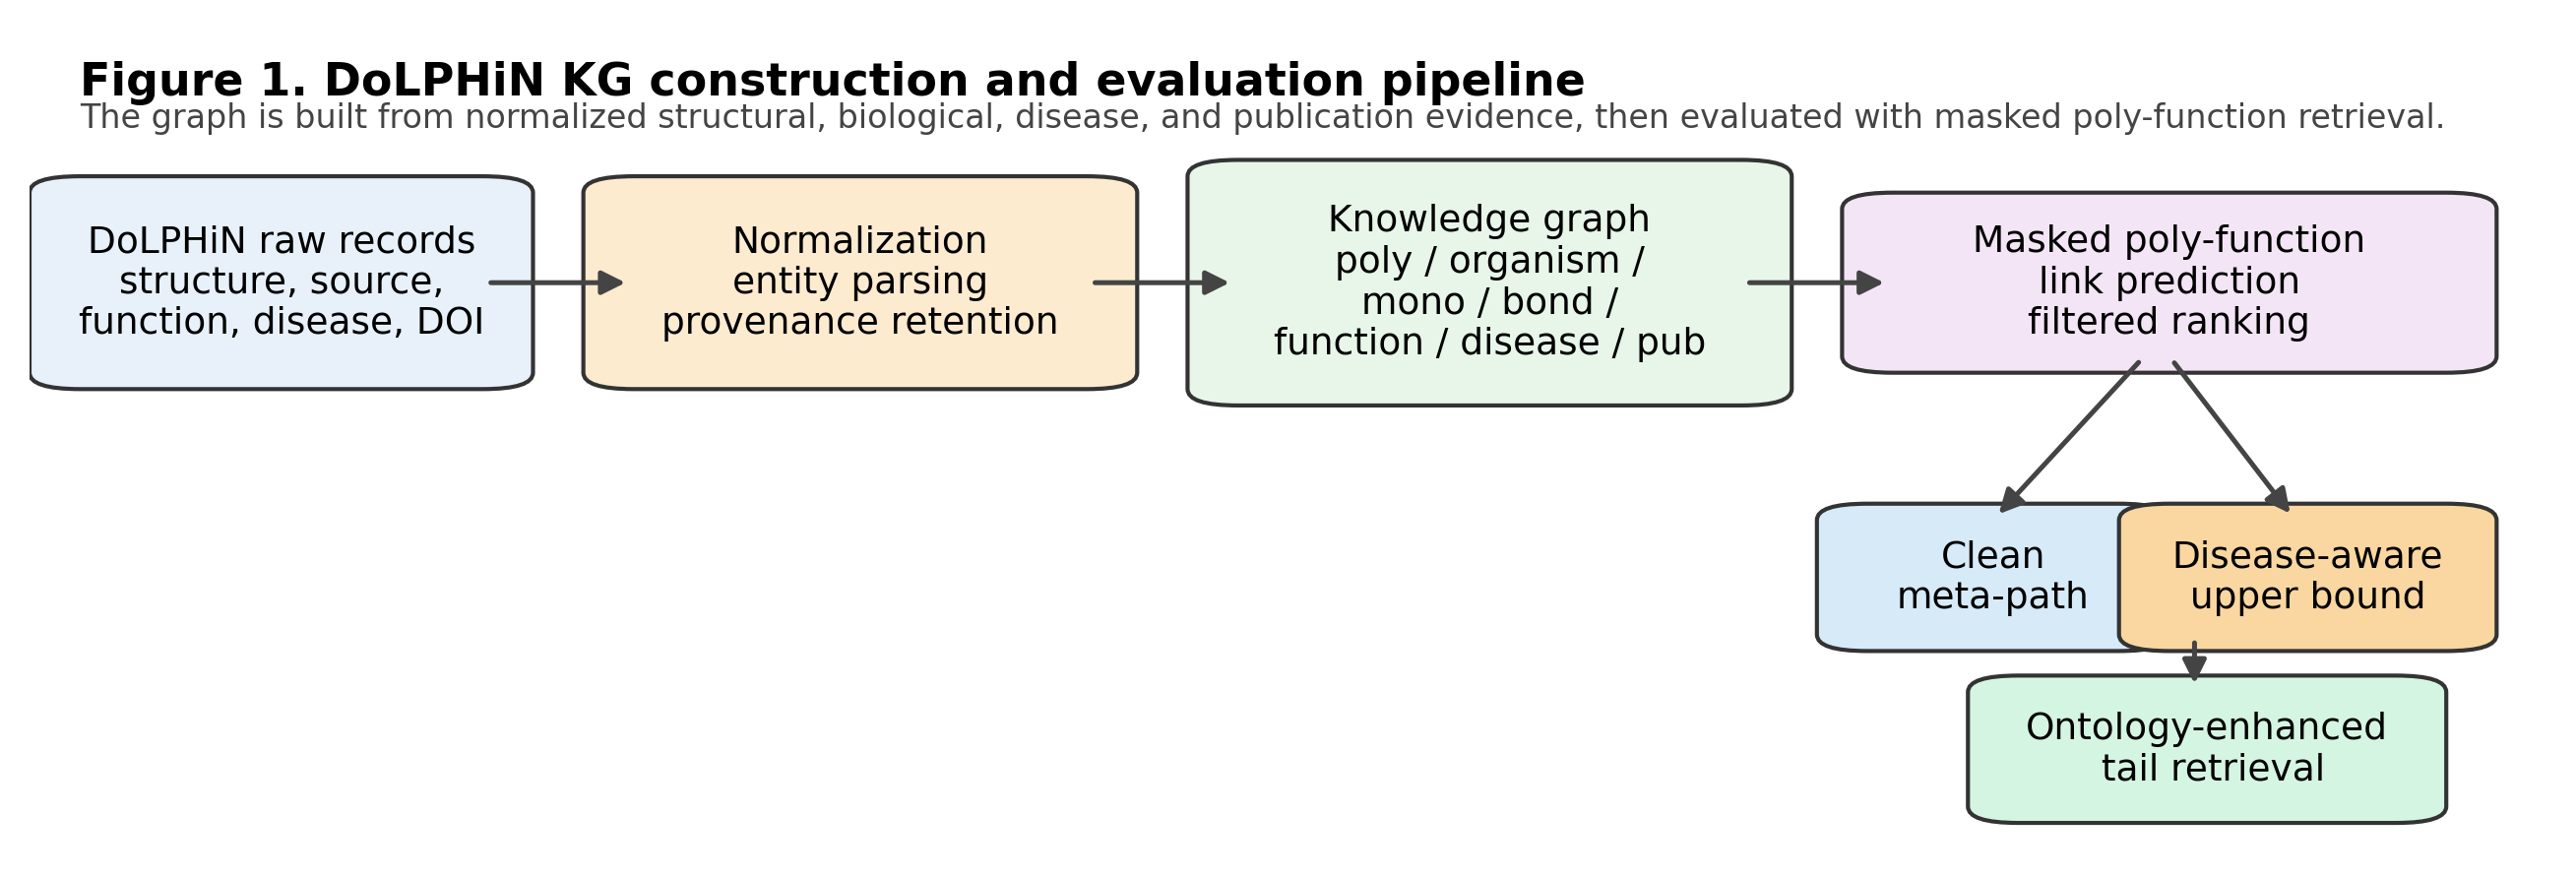
\includegraphics[width=0.96\textwidth]{../../paper/figures/figure1_pipeline.png}
\caption{DoLPHiN KG construction and evaluation pipeline. Raw DoLPHiN records are normalized into typed entities and relations spanning polysaccharides, organisms, monosaccharides, glycosidic bonds, functions, diseases, and publications. The resulting graph supports masked \texttt{poly-function} link prediction under filtered ranking. The paper studies three settings on top of the same graph substrate: clean meta-path retrieval, disease-aware upper-bound retrieval, and ontology-enhanced tail-sensitive retrieval.}
\label{fig:pipeline}
\end{figure*}

\section{Materials and Methods}
\label{sec:methods}

We build a heterogeneous knowledge graph centered on \texttt{Polysaccharide} entities extracted from DoLPHiN. Each polysaccharide node is linked to normalized \texttt{Organism}, \texttt{Monosaccharide}, \texttt{GlycosidicBond}, \texttt{Function}, \texttt{Disease}, and \texttt{Publication} nodes. The current graph contains 5,078 polysaccharides, 1,487 organism nodes, 23 monosaccharide nodes, 323 glycosidic bond nodes, 66 function nodes, 14 disease nodes, and 2,386 publication nodes. The resulting graph preserves both typed structure and record-level provenance, which allows the same resource to support querying, graph export, and controlled predictive evaluation. The graph statistics are summarized in Table~\ref{tab:kg-summary}.

\subsection{KG Construction and Normalization}
\label{sec:kg-construction}

The KG is built from DoLPHiN-centered JSONL records through a normalization-first ETL process. Each record contributes exactly one polysaccharide identifier, while the free-text fields describing source organism, monomer composition, glycosidic linkage, functional annotations, disease associations, and DOI metadata are converted into typed node and edge tables. The normalization layer is intentionally conservative. We merge entities only when they map to the same canonical normalized string within a node type; otherwise we preserve the original distinction and keep the source record link for traceability. This design prevents overly aggressive collapsing of biologically distinct but lexically similar terms.

The normalization rules differ by field. Organism strings are normalized into organism nodes and accompanied by lightweight taxonomy attributes used later for source-aware retrieval. Monomer composition strings are parsed into normalized monosaccharide entities and attached to polysaccharides through composition edges. Linkage strings are converted into glycosidic bond signatures rather than being left as raw text tokens. Functional labels and disease strings are normalized into graph nodes, but the original record-level provenance is retained so that each predicted edge can still be traced back to the originating DoLPHiN record and DOI. Publication nodes currently use DOI as the primary normalized identifier, which is why they are suitable for provenance tracking but not yet for full bibliometric analysis.

Missing information is handled by omission rather than imputation. If a record lacks a particular normalized field, no edge of that type is created, and the absence is treated as missing evidence rather than negative evidence. Duplicate node identifiers are checked during export, and edge validation is performed against the final node tables. The current graph passes this validation without broken references, which reduces the risk that downstream retrieval performance is being influenced by malformed graph structure rather than model behavior.

\subsection{Function Hierarchy Construction}
\label{sec:hierarchy-construction}

The ontology used in the long-tail experiments is not intended as a comprehensive biological ontology of polysaccharide function. Instead, it is a task-oriented hierarchy constructed over the DoLPHiN function label set. The final hierarchy contains 11 intermediate function families and 11 parent-to-family edges, with the family-to-label mapping listed in Supplementary Table S3. Earlier family-only formulations were too coarse and tended either to have no effect or to oversmooth function groups. We therefore converted the hierarchy into explicit parent/child relations, where each child label inherits only from a small set of semantically broader parent categories. This parent/child graph is used only in the ontology-enhanced retrieval variants and is never mixed into the clean baseline.

The hierarchy design follows two constraints. First, each parent/child relation must be interpretable enough to justify evidence propagation between labels. Second, the hierarchy must remain sparse enough that propagation does not become a synonym for global smoothing. These constraints are operationalized through the confidence-gated parent/child propagation rule described below: ontology evidence is allowed to intervene only when local support is limited and when the parent region is sufficiently seeded by nearby candidates.

\subsection{Evaluation Protocol}
\label{sec:evaluation-protocol}

Our primary task is masked \texttt{poly-function} link prediction. For each evaluation instance, one known \texttt{Polysaccharide}-to-\texttt{Function} edge is hidden, and the model ranks all candidate function nodes for that polysaccharide. We report filtered ranking so that other true functions already attached to the same polysaccharide are removed from the candidate set before rank computation. This is essential because the task is intrinsically multi-label: a polysaccharide can legitimately connect to several true functions, and those additional true edges should not be counted as ranking errors when one edge is masked.

We use two complementary evaluation views. The first is a single tuned split, which is used for the headline baseline comparison in Tables~\ref{tab:clean-diagnostic} and~\ref{tab:retrieval-results}. The second is a paired multi-seed protocol used specifically for stability and significance analysis of the ontology variant. In that protocol, baseline and ontology runs share the same random seed and the same masked edges, so the statistical unit is a paired edge-level comparison rather than an unpaired aggregate metric. This distinction is important because the tuned-split result and the pooled paired-seed result answer different questions: the former reports the best representative operating point, while the latter estimates whether the observed tail gain remains consistent under repeated paired evaluation. Throughout the paper, we treat the paired 16-seed protocol as the primary evidence for ontology stability and the tuned split only as an interpretable operating point.

To avoid aggregate metrics being dominated by common labels, we stratify evaluation by training-label support. Labels with training support between 1 and 10 are treated as tail, support between 11 and 50 as mid, and support above 50 as head. These thresholds are not intended as universal biological categories; they are evaluation strata chosen to separate the extremely data-sparse regime from the moderately supported and heavily supported regimes. In the paired significance analysis, we report both two-sided and directional one-sided tests. The one-sided test is used only for the tail-sensitive ontology claim because that intervention is explicitly designed to improve low-support retrieval rather than to maximize a symmetric global metric.

We also separate clean and disease-aware settings throughout the paper. The clean setting asks whether graph structure alone provides usable function signal. The disease-aware setting instead estimates an upper bound when auxiliary disease semantics are available. Because disease is strongly coupled to function labels in DoLPHiN, these settings should not be interpreted as interchangeable. This separation is part of the leakage-control logic of the paper: disease-aware results are reported as semantically enriched upper-bound retrieval rather than as the primary structure-only claim.

\subsection{Leakage Control and Information Boundaries}
\label{sec:leakage-control}

The main leakage-control principle is that an observed edge is never allowed to remain in the candidate set as a visible positive during evaluation. For masked \texttt{poly-function} prediction, the held-out function edge is removed before ranking, and filtered ranking additionally removes the same polysaccharide's other true function labels from the error set. This prevents the multi-label setting from artificially penalizing a model for retrieving a different true label attached to the same query node.

Potential information leakage is handled differently depending on the relation type. In the clean setting, disease-derived features and edges are excluded entirely, because they are too tightly coupled to the target functions to support a clean structure-only claim. In the disease-aware setting, they are reintroduced explicitly and are interpreted as auxiliary semantics rather than as part of the main biological mechanism. Organism, monosaccharide, bond, and publication relations are retained in both settings because they are part of the intended typed-evidence graph. However, publication is currently represented only through DOI-level provenance and is not used as an independent textual evidence encoder, which reduces the risk that the model is simply memorizing literature descriptions instead of graph relations. Finally, graph export validation confirms that all edge tables resolve to existing node identifiers, so performance differences are not attributable to malformed graph connectivity.

In addition to the retrieval models used for masked link prediction, we evaluate a unified family of clean function-prediction baselines on the same train/valid/test split. The feature blocks come from two sources. The first is the exported polysaccharide feature vector (\texttt{poly\_x}), which contains numeric structural summaries produced during graph export and is also the base node-local input to the neural baselines. The second is an explicit sparse meta-path incidence vector built from organism, monosaccharide, glycosidic bond, and publication relations. We evaluate three shallow classifiers over these feature spaces: regularized one-vs-rest logistic regression, a linear SGD surrogate, and a shallow multilayer perceptron. Validation thresholds are tuned per label and then reused for the test split. These models are intended to answer a concrete benchmarking question: if explicit typed evidence is already available, how much of the clean signal can be recovered without message passing?

For neural baselines, we use a two-layer hetero GraphSAGE model on the exported PyG graph and a hybrid variant that concatenates the same sparse meta-path block to the polysaccharide node input. To isolate whether message passing itself contributes meaningful signal, we add paired failure ablations: a \texttt{hetero\_no\_message} model that preserves the same training loop but removes graph aggregation, and \texttt{poly\_mlp} models that operate only on node-local inputs. This design makes the shallow-versus-neural comparison diagnostic rather than adversarial: the strongest shallow model and the hybrid GNN both see the same main typed evidence blocks, but one consumes them directly while the other asks message passing to add value on top of them. If the full hetero model and the no-message ablation are nearly identical, then the missing ingredient is not simply another round of learning-rate or depth tuning; it is the graph evidence available to message passing.

The disease-aware retrieval models are evaluated as upper-bound settings, where disease-conditioned compatibility is injected into the retrieval stage and then mildly frequency-adjusted to reduce the bias toward frequent labels.

To target the long tail, we introduce ontology-aware parent/child propagation. A manually curated function hierarchy is represented as directed parent/child relations rather than undifferentiated family membership. During retrieval, the base disease-aware score first forms a shortlist of plausible function labels. Ontology propagation is then activated only when the local evidence is sufficiently uncertain and when there is enough seed support in the relevant parent region. The propagated contribution is further modulated by an adaptive confidence gate, preventing coarse family smoothing from overwhelming the original neighborhood evidence. This design is motivated by our earlier failures with hierarchy bonuses and family-level smoothing, which either had negligible effect or degraded overall ranking. Figure~\ref{fig:pipeline} highlights where ontology enters the pipeline: not as a post-hoc family bonus, but as selective evidence propagation inside the retrieval stage.

All experiments are implemented in the project release accompanying this manuscript. The release package contains the normalized KG export, the unified split definition, the task-specific function hierarchy configuration, the paired edge-level ontology stability records, and the benchmark scripts for graph construction, retrieval, shallow baselines, and GNN ablations. The current implementation uses Python 3.9 with PyTorch and PyTorch Geometric for graph models and scikit-learn for shallow baselines. We will expose these artifacts in the public repository and supplementary package at submission time so that the full benchmark can be re-run from the released configuration files rather than reconstructed from prose alone.

\section{Results}
\label{sec:experiments}

We first evaluate whether the graph is useful for clean function prediction at all under a unified train/valid/test split. The answer is yes, but the strongest evidence comes from explicit shallow feature models rather than from the current GNN stack. After removing disease-derived degree information from the clean \texttt{poly\_x} export, a regularized one-vs-rest logistic model on meta-path incidence features is the strongest clean diagnostic baseline, with test macro-F1 0.3465 and exact match 0.5118. Concatenating the corrected disease-free \texttt{poly\_x} block with meta-path features reaches 0.3317 macro-F1 and 0.5059 exact match. A shallow MLP on the same meta-path features is weaker at 0.3065, showing that the main gain does not come from replacing a linear decision boundary with a generic neural classifier. By contrast, the clean hetero GNN and node-local neural ablations remain far lower, around 0.04--0.05 macro-F1. This result sharpens the clean claim of the paper: the current DoLPHiN-derived graph already supports useful structure-only prediction, but the useful signal is more accessible through explicit typed feature blocks than through the current hetero message-passing formulation. Figure~\ref{fig:benchmarks}A provides the comparative pattern, and Table~\ref{tab:clean-diagnostic} gives the exact values.

We next ask whether the poor GNN performance is mainly an optimization issue or a representation issue. The failure ablation strongly favors the second explanation. On the corrected clean base graph, the full hetero GraphSAGE model reaches 0.0464 test macro-F1, the no-message ablation reaches 0.0426, and a \texttt{poly\_mlp} baseline on the same exported node features reaches 0.0466. This is the key mechanistic result behind the benchmark table: on the present graph, message passing is not adding useful incremental evidence beyond what is already contained in node-local inputs, so the current bottleneck should be interpreted as a representation mismatch rather than as a simple tuning deficit. Figure~\ref{fig:benchmarks}C provides the failure pattern, and Table~\ref{tab:gnn-ablation} provides the exact numerical comparison.

We then turn to masked \texttt{poly-function} link prediction, which is the primary retrieval benchmark of the paper. The main disease-aware baseline is the disease-conditioned vote combined with a frequency-adjusted disease prior. This baseline is strong in aggregate ranking, but support-stratified analysis reveals a persistent long-tail weakness. A large set of long-tail interventions was tested, including rare-label neighbor expansion, source-constrained reranking, structure-aware candidate generation, motif-based signatures, and several ontology variants. Most either failed to change the shortlist or traded away head performance without improving the tail. This negative evidence is important because it narrows the plausible mechanisms: the tail problem is not solved by stronger family smoothing or by generic structural bonuses. The disease-aware retrieval comparison and the tuned ontology result are shown in Figure~\ref{fig:benchmarks}B.

The useful ontology mechanism is the confidence-gated parent/child propagation model. On the representative tuned split, it preserves the disease-aware upper bound almost exactly, with filtered MRR moving from 0.8491 to 0.8490, Hits@3 staying at 0.912, and Hits@5 moving from 0.938 to 0.939, while improving tail micro filtered Hits@3 from 0.1667 to 0.3333. To determine whether this effect is stable rather than accidental, we ran a paired significance protocol over 16 seeds, yielding 16,000 masked edges with edge-level records for both the baseline and the ontology variant. Under this pooled paired protocol, global aggregate ranking changes are statistically detectable in some metrics but practically negligible in effect size: filtered Hits@3 moves from 0.9088 to 0.9085, filtered Hits@5 stays at 0.9366, and the filtered MRR delta is only $-0.0003$. However, the tail-sensitive gains remain consistent: tail micro filtered Hits@3 increases from 0.0552 to 0.1021, the directional one-sided McNemar test gives p = 0.03125, and the tail filtered MRR gain is 0.0395 with permutation p = 0.0002499. No seed shows a tail regression. Figure~\ref{fig:stability} presents the seed-level non-regression pattern and the paired significance summary, while Table~\ref{tab:stability} lists the corresponding numerical results.

\subsection{Biological Case Studies}
\label{sec:biological-case-studies}

The aggregate metrics become easier to trust when they are connected back to concrete local evidence. We therefore built a case-study pool from edge-level evaluation records and enriched each candidate with the corresponding organism, monosaccharide, bond, disease, and DOI evidence from the final KG before selecting manuscript-facing examples. This avoids choosing illustrative cases directly from headline tables and keeps the qualitative interpretation aligned with the actual retrieval protocol. Supplementary Table S1 summarizes the selected manuscript-facing cases and their supporting evidence channels.

The first useful pattern is that clean retrieval can already succeed when the typed local evidence is coherent. In the clean benchmark, \texttt{BEP} recovers \texttt{immunomodulatory} at filtered rank 1, and \texttt{Galactofucan(M05 RDP 2H)} recovers \texttt{anticoagulant} at filtered rank 1. These examples are important because they show that the clean graph is not merely weakly informative in aggregate. Instead, the graph already contains biologically interpretable evidence chains anchored in source organism, monosaccharide composition, linkage signatures, and DOI-linked provenance. The BEP case is anchored to an experimentally characterized \textit{Boletus edulis} polysaccharide with reported immunomodulatory and antitumor activity~\cite{wang2014boletus}; the galactofucan case is anchored to a brown-seaweed polysaccharide characterization study~\cite{rioux2010galactofucan}. This is consistent with the strong performance of the shallow explicit-feature baselines: the useful signal is present, but it is concentrated in typed local evidence blocks rather than in the deeper neighborhoods that the current GNNs attempt to aggregate.

The second useful pattern is that the ontology claim is highly selective rather than global. The clearest ontology-rescued tail case is \texttt{APP90-2}, where the held-out \texttt{osteogenic} label has training support 2. Under the disease-aware baseline this label appears only at filtered rank 43, whereas confidence-gated parent/child propagation moves it to filtered rank 3. This case is biologically plausible because APP90-2 is linked to a reported osteogenic polysaccharide from \textit{Alhagi pseudalhagi}~\cite{ye2021app90}. Figure~\ref{fig:case-subgraphs} visualizes this rescue together with a representative persistent failure. In the failure case, \texttt{CZGS-1} with held-out \texttt{antiinflammatory} already carries rich local evidence from an \textit{Amygdalus scoparia} gum polysaccharide characterization study~\cite{molaei2018czgs}, yet remains at rank 12 in the clean setting and rank 19 in both the disease-aware baseline and ontology-enhanced variant. The contrast between these two cases clarifies the boundary of the method: ontology can selectively reroute evidence for some low-support labels, but it does not compensate for missing motif-level structure or for local evidence that is insufficiently discriminative.

\begin{figure*}[t]
\centering
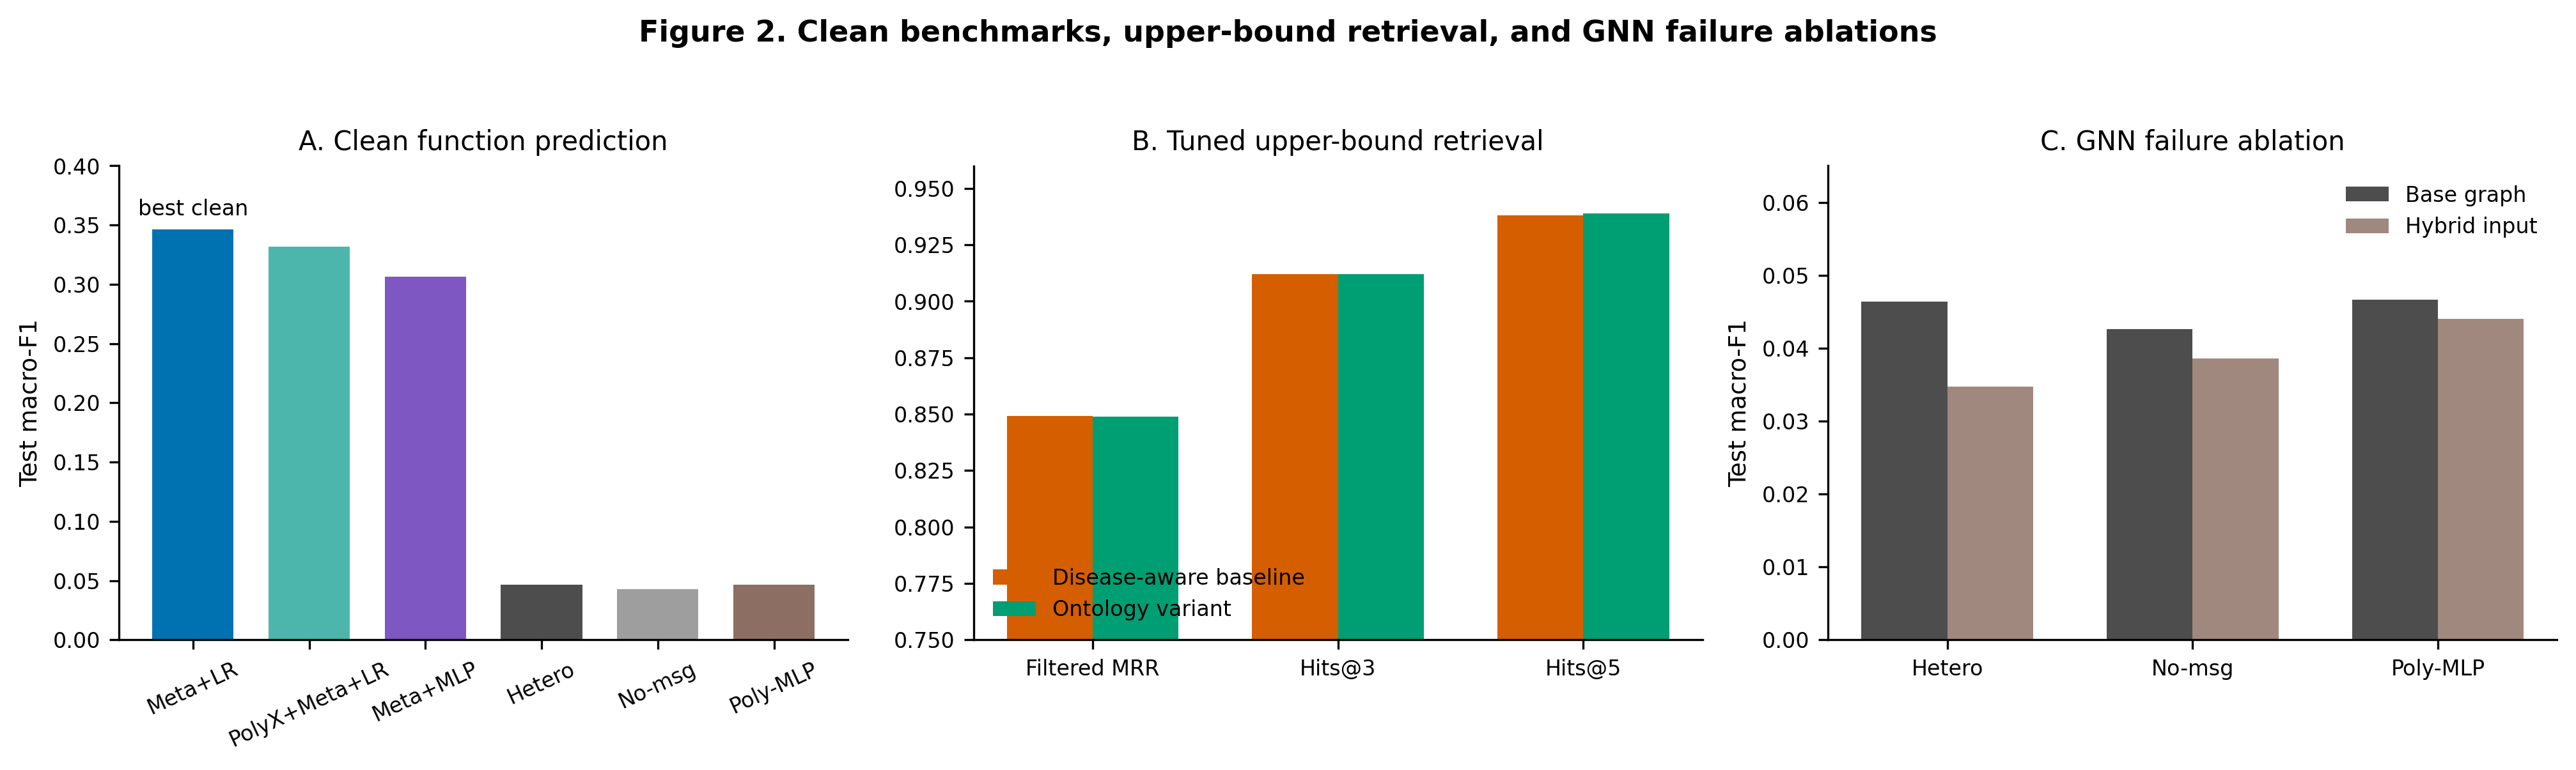
\includegraphics[width=0.96\textwidth]{../../paper/figures/figure2_benchmarks.png}
\caption{Clean benchmarks, upper-bound retrieval, and GNN failure ablations. Panel A compares clean function-prediction baselines under the unified split, showing that the strongest model is a shallow linear classifier on explicit graph features rather than a neural message-passing model. Panel B compares the tuned disease-aware retrieval baseline against the ontology-enhanced variant on filtered MRR, Hits@3, and Hits@5. Panel C summarizes the GNN failure ablation, showing that no-message variants remain close to the full hetero models.}
\label{fig:benchmarks}
\end{figure*}

\begin{table*}[t]
\centering
\caption{Summary statistics of the DoLPHiN-derived knowledge graph. The graph contains typed structural, biological, functional, disease, and publication evidence derived from normalized DoLPHiN records.}
\label{tab:kg-summary}
\begin{tabular}{lc}
\toprule
Entity or relation type & Count \\
\midrule
Polysaccharide nodes & 5,078 \\
Organism nodes & 1,487 \\
Monosaccharide nodes & 23 \\
Glycosidic bond nodes & 323 \\
Function nodes & 66 \\
Disease nodes & 14 \\
Publication nodes & 2,386 \\
Polysaccharide-organism edges & 5,075 \\
Polysaccharide-monosaccharide edges & 17,448 \\
Polysaccharide-bond edges & 2,313 \\
Polysaccharide-function edges & 7,408 \\
Polysaccharide-disease edges & 3,633 \\
Polysaccharide-publication edges & 5,071 \\
\bottomrule
\end{tabular}
\end{table*}

\begin{table*}[t]
\centering
\caption{Clean diagnostic function-prediction results on the unified split. All rows exclude disease-derived features and use the corrected clean PyG payload whose polysaccharide feature schema contains zero disease-derived fields. Higher macro-F1 and exact match are better.}
\label{tab:clean-diagnostic}
\begin{tabularx}{\textwidth}{>{\raggedright\arraybackslash}p{3.2cm}>{\raggedright\arraybackslash}p{3.0cm}>{\centering\arraybackslash}p{1.8cm}>{\centering\arraybackslash}p{1.8cm}>{\raggedright\arraybackslash}X}
\toprule
Model & Feature input & Macro-F1 $\uparrow$ & Exact match $\uparrow$ & Note \\
\midrule
Meta-path + LogReg & organism / monosaccharide / bond / publication meta-paths & \best{0.3465} & 0.5118 & strongest clean baseline \\
Poly-X + Meta-path + LogReg & corrected disease-free \texttt{poly\_x} + meta-paths & 0.3317 & 0.5059 & \texttt{poly\_x} no longer contains disease degree \\
Meta-path + MLP & meta-paths & 0.3065 & \best{0.5295} & neural shallow baseline \\
Hetero GNN & corrected clean graph & 0.0464 & 0.0138 & message passing baseline \\
Poly-MLP & corrected disease-free \texttt{poly\_x} & 0.0466 & 0.0197 & node-local neural baseline \\
\bottomrule
\end{tabularx}
\end{table*}

\begin{table*}[t]
\centering
\caption{Representative tuned split for masked \texttt{poly-function} retrieval. Disease-aware retrieval is treated as an upper-bound semantic setting. The ontology row reports the best tuned ontology-enhanced variant on that same split and should be interpreted as a tail-sensitive supplement rather than as a new overall best model. These values are not directly comparable to the pooled paired-seed statistics in Table~\ref{tab:stability}. Higher values are better.}
\label{tab:retrieval-results}
\begin{tabularx}{\textwidth}{>{\raggedright\arraybackslash}p{2.6cm}>{\raggedright\arraybackslash}p{1.8cm}>{\centering\arraybackslash}p{1.6cm}>{\centering\arraybackslash}p{1.3cm}>{\centering\arraybackslash}p{1.3cm}>{\centering\arraybackslash}p{1.6cm}>{\raggedright\arraybackslash}X}
\toprule
Model & Setting & Filtered MRR $\uparrow$ & Hits@3 $\uparrow$ & Hits@5 $\uparrow$ & Tail Hits@3 $\uparrow$ & Note \\
\midrule
Disease-aware baseline & upper bound & \best{0.8491} & 0.912 & 0.938 & 0.1667 & disease vote + frequency prior \\
Ontology best variant & tail-sensitive & 0.8490 & 0.912 & \best{0.939} & \best{0.3333} & gated parent/child propagation \\
\bottomrule
\end{tabularx}
\end{table*}

\begin{table*}[t]
\centering
\caption{GNN failure ablation under the leakage-controlled clean unified split. All rows use the corrected clean PyG payload whose polysaccharide features contain no disease-derived fields. Message-passing remains close to no-message and node-local controls, indicating that the current bottleneck is graph representation rather than a missing training trick.}
\label{tab:gnn-ablation}
\begin{tabularx}{\textwidth}{>{\raggedright\arraybackslash}p{2.2cm}>{\raggedright\arraybackslash}p{2.2cm}>{\raggedright\arraybackslash}p{1.9cm}XXX}
\toprule
Input graph & Model & Protocol & Metric 1 & Metric 2 & Note \\
\midrule
Base & Hetero GNN & seed 42 & Macro-F1 0.0464 & Exact match 0.0138 & full message passing \\
Base & No-message ablation & seed 42 & Macro-F1 0.0426 & Exact match 0.0315 & no material gain from propagation \\
Base & Poly-MLP & seed 42 & Macro-F1 0.0466 & Exact match 0.0197 & node-local neural baseline \\
\bottomrule
\end{tabularx}
\end{table*}

\section{Discussion}
\label{sec:discussion}

The results indicate that the immediate value of the DoLPHiN-derived knowledge graph lies in structured retrieval and explicit typed feature models rather than in the current generation of graph neural architectures. This does not imply that GNNs are unsuitable for polysaccharide graphs in principle. Instead, it suggests that the present graph version exposes stronger signal through explicit relation structure than through shallow neighborhood aggregation. Non-polysaccharide nodes remain semantically weak, graph connectivity is sparse relative to the prediction difficulty, and several critical structural regularities are more naturally expressed as typed evidence blocks than as messages propagated through weakly featured neighbors. In that sense, the present paper is better understood as a KG resource and benchmark diagnosis paper than as a claim that graph neural modeling has been exhausted for this domain.

The disease-aware results should also be interpreted carefully. They demonstrate that disease information is strongly predictive, but this is precisely why it should not define the clean main claim. If disease is tightly coupled to the target function labels, then disease-aware retrieval is better understood as an upper-bound semantic enhancement. Our cleaner scientific claim is therefore that the knowledge graph already supports useful function retrieval without disease, while disease and ontology help explain where additional side information can be injected and how that affects the long tail. For the ontology component specifically, we treat the paired 16-seed analysis as the primary evidence of stability, and the tuned split only as a representative operating point.

The GNN failure ablations are especially useful because they constrain what future model work should prioritize. The full hetero GNN and no-message controls are nearly indistinguishable, which means the next step is not simply a deeper or more heavily tuned message-passing stack. More promising directions are richer non-polysaccharide node semantics, motif-level or subgraph-level encoders, and retrieval-guided graph models that can preserve high-signal local structure instead of diffusing it. We also avoid over-interpreting exact-match differences in these ablations: in this multi-label setting, exact match is brittle and can look deceptively large when a model predicts very sparse label sets, even while macro-F1 remains poor.

The ontology findings are also instructive because they constrain future work. Coarse family bonuses and undirected hierarchy smoothing were ineffective. Parent/child propagation became useful only when it was selective, confidence-gated, and integrated directly into retrieval rather than appended as a generic reranking bonus. This pattern suggests that ontology in this domain is most valuable as a targeted evidence-routing mechanism for under-supported labels, not as a broad semantic regularizer. We therefore interpret the ontology result as proof-of-principle tail intervention on a task-specific hierarchy rather than as a comprehensive ontology-learning result. A practical next step is therefore not to enlarge the ontology blindly, but to refine local parent/child evidence and combine it with richer structural signatures that are currently absent from the graph.

The biology-facing case studies help translate these technical findings into evidence patterns that are easier to inspect. The clean success cases show that the graph can already support plausible function retrieval through local typed evidence chains anchored in source organism, composition, and bond signatures. The ontology-rescued \texttt{APP90-2}/\texttt{osteogenic} case then shows what a successful ontology intervention actually looks like: not a global semantic smoother, but a narrow parent/child route that helps a low-support label cross the top-ranked boundary. Conversely, the persistent \texttt{CZGS-1}/\texttt{antiinflammatory} failure shows that even a richly connected local neighborhood may remain insufficient when the missing signal lies in finer structural motifs or provenance semantics that the current graph does not encode. For that reason, we interpret the ontology result as a selective tail-sensitive mechanism rather than as a comprehensive biological solution.

\subsection{Related context}
\label{sec:related-work}

Existing work relevant to this study falls into three partially overlapping groups. The first group concerns polysaccharide databases and glycan resources. Resources such as GlyTouCan, GlyCosmos, CSDB, and more recent polysaccharide-centered databases have substantially improved glycan curation, interoperability, and browsing~\cite{aoki2016glytoucan,yamada2020glycosmos,toukach2015csdb,xin2025dolphin}. These resources are indispensable for curation and lookup, but they are usually optimized for record access rather than for graph-native retrieval benchmarks. Our work differs in emphasis: the objective is not only to store polysaccharide records, but to normalize them into a typed evidence graph that can support controlled predictive tasks with provenance preserved.

The second group covers knowledge-graph-based biological prediction. In many biomedical settings, graph learning has been used to connect heterogeneous entities such as molecules, diseases, genes, phenotypes, and publications~\cite{zhou2020biomedicalkg,chandak2023primekg,crichton2018linkprediction,gema2024kgembeddings,zhao2024community}. The dominant intuition in that literature is that richer heterogeneous connectivity should favor graph neural models or embedding-based reasoning. Our results only partly align with that expectation. On the current DoLPHiN-derived graph, explicit relation-derived retrieval remains stronger than the hetero GNN baselines, which suggests that graph-native biological prediction should not automatically be equated with end-to-end message passing. In sparse and weakly featured scientific graphs, interpretable retrieval may still be the more faithful first-line model.

The third group concerns ontology-aware reasoning and long-tail prediction. Ontologies and hierarchies are often used as label regularizers, smoothers, or knowledge-transfer structures in long-tailed classification~\cite{li2021hierarchical,liu2024multigranularity}. Our experiments show that these generic formulations are not sufficient in the present setting. Family-level bonuses and coarse hierarchy smoothing were ineffective or harmful. The effective ontology formulation is narrower: parent/child relations must be injected as selective evidence propagation under confidence control. This places our work closer to targeted tail-sensitive calibration than to generic ontology regularization.

\begin{figure*}[t]
\centering
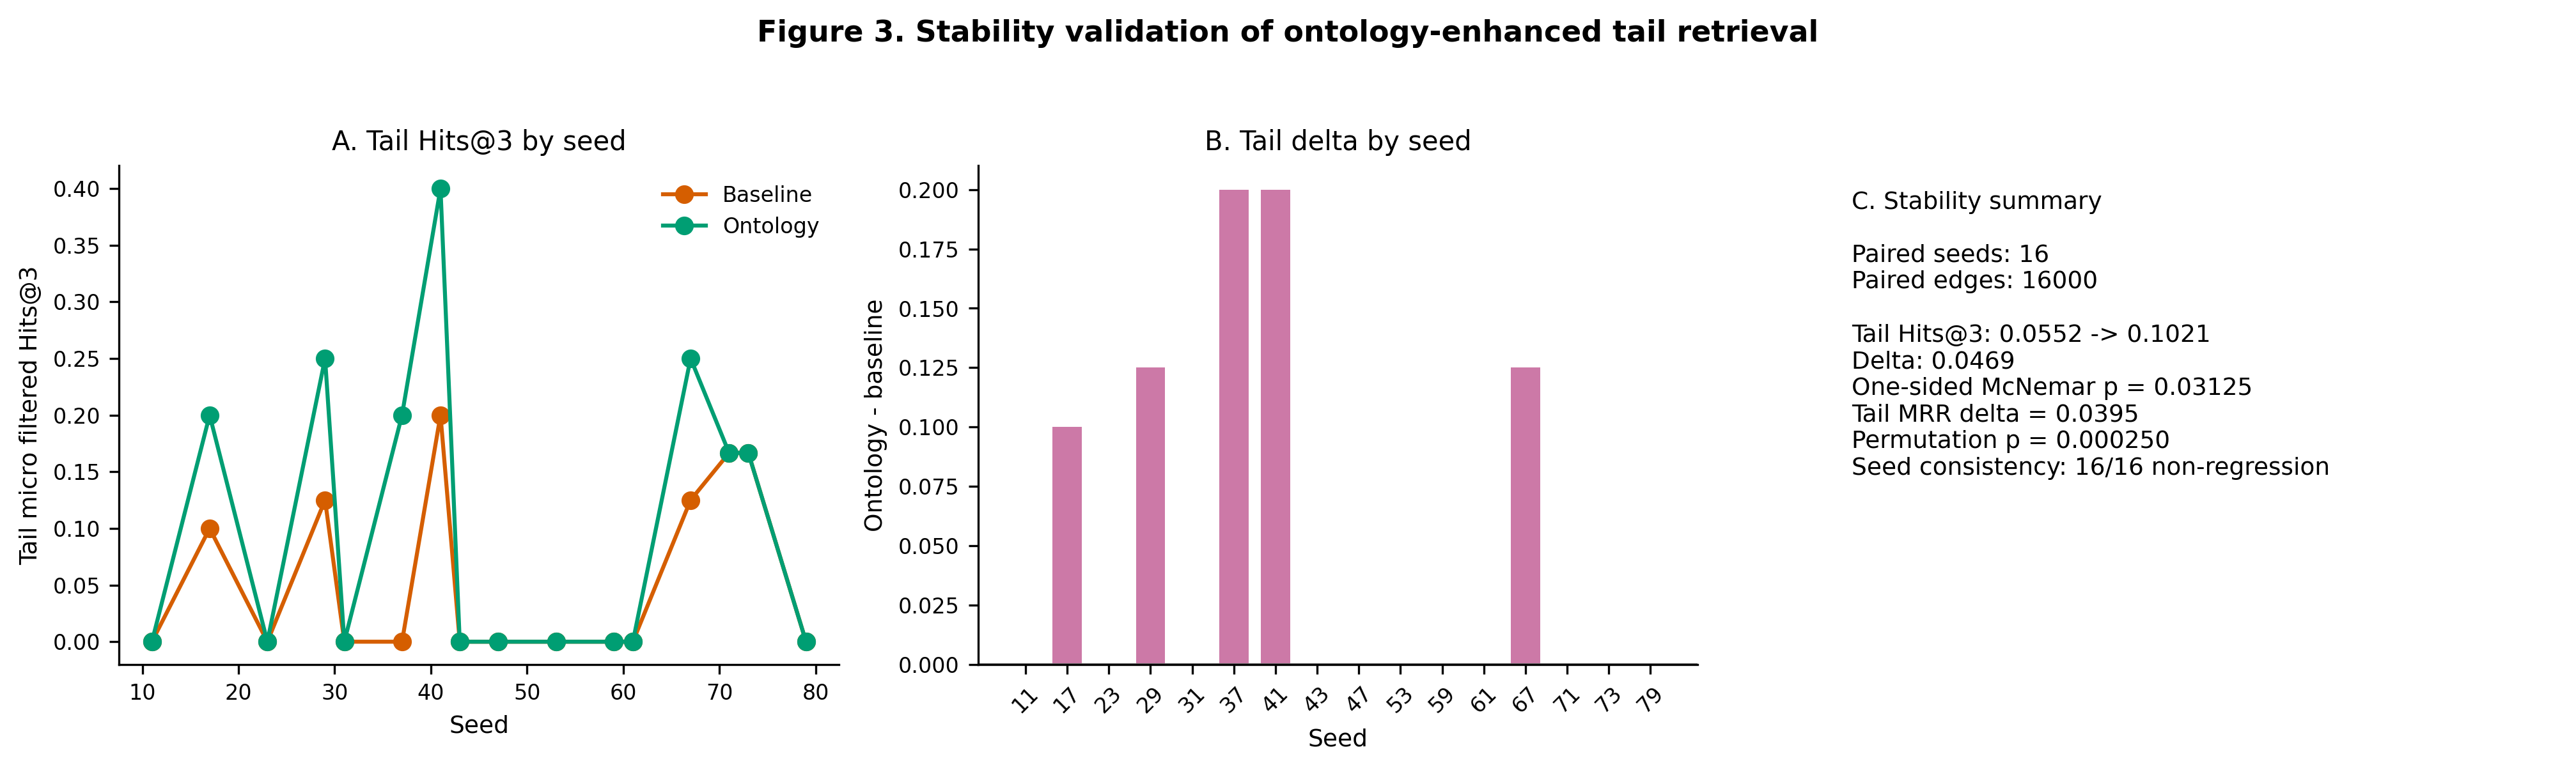
\includegraphics[width=0.96\textwidth]{../../paper/figures/figure3_stability.png}
\caption{Stability validation for ontology-enhanced tail retrieval. Panel A shows paired seed-wise tail micro filtered Hits@3 for the disease-aware baseline and the ontology-enhanced variant. Panel B shows the per-seed ontology-minus-baseline delta. Panel C summarizes the paired statistical tests, indicating that ontology-enhanced propagation yields a stable tail-sensitive gain with no observed tail regression across seeds.}
\label{fig:stability}
\end{figure*}

\begin{figure*}[t]
\centering
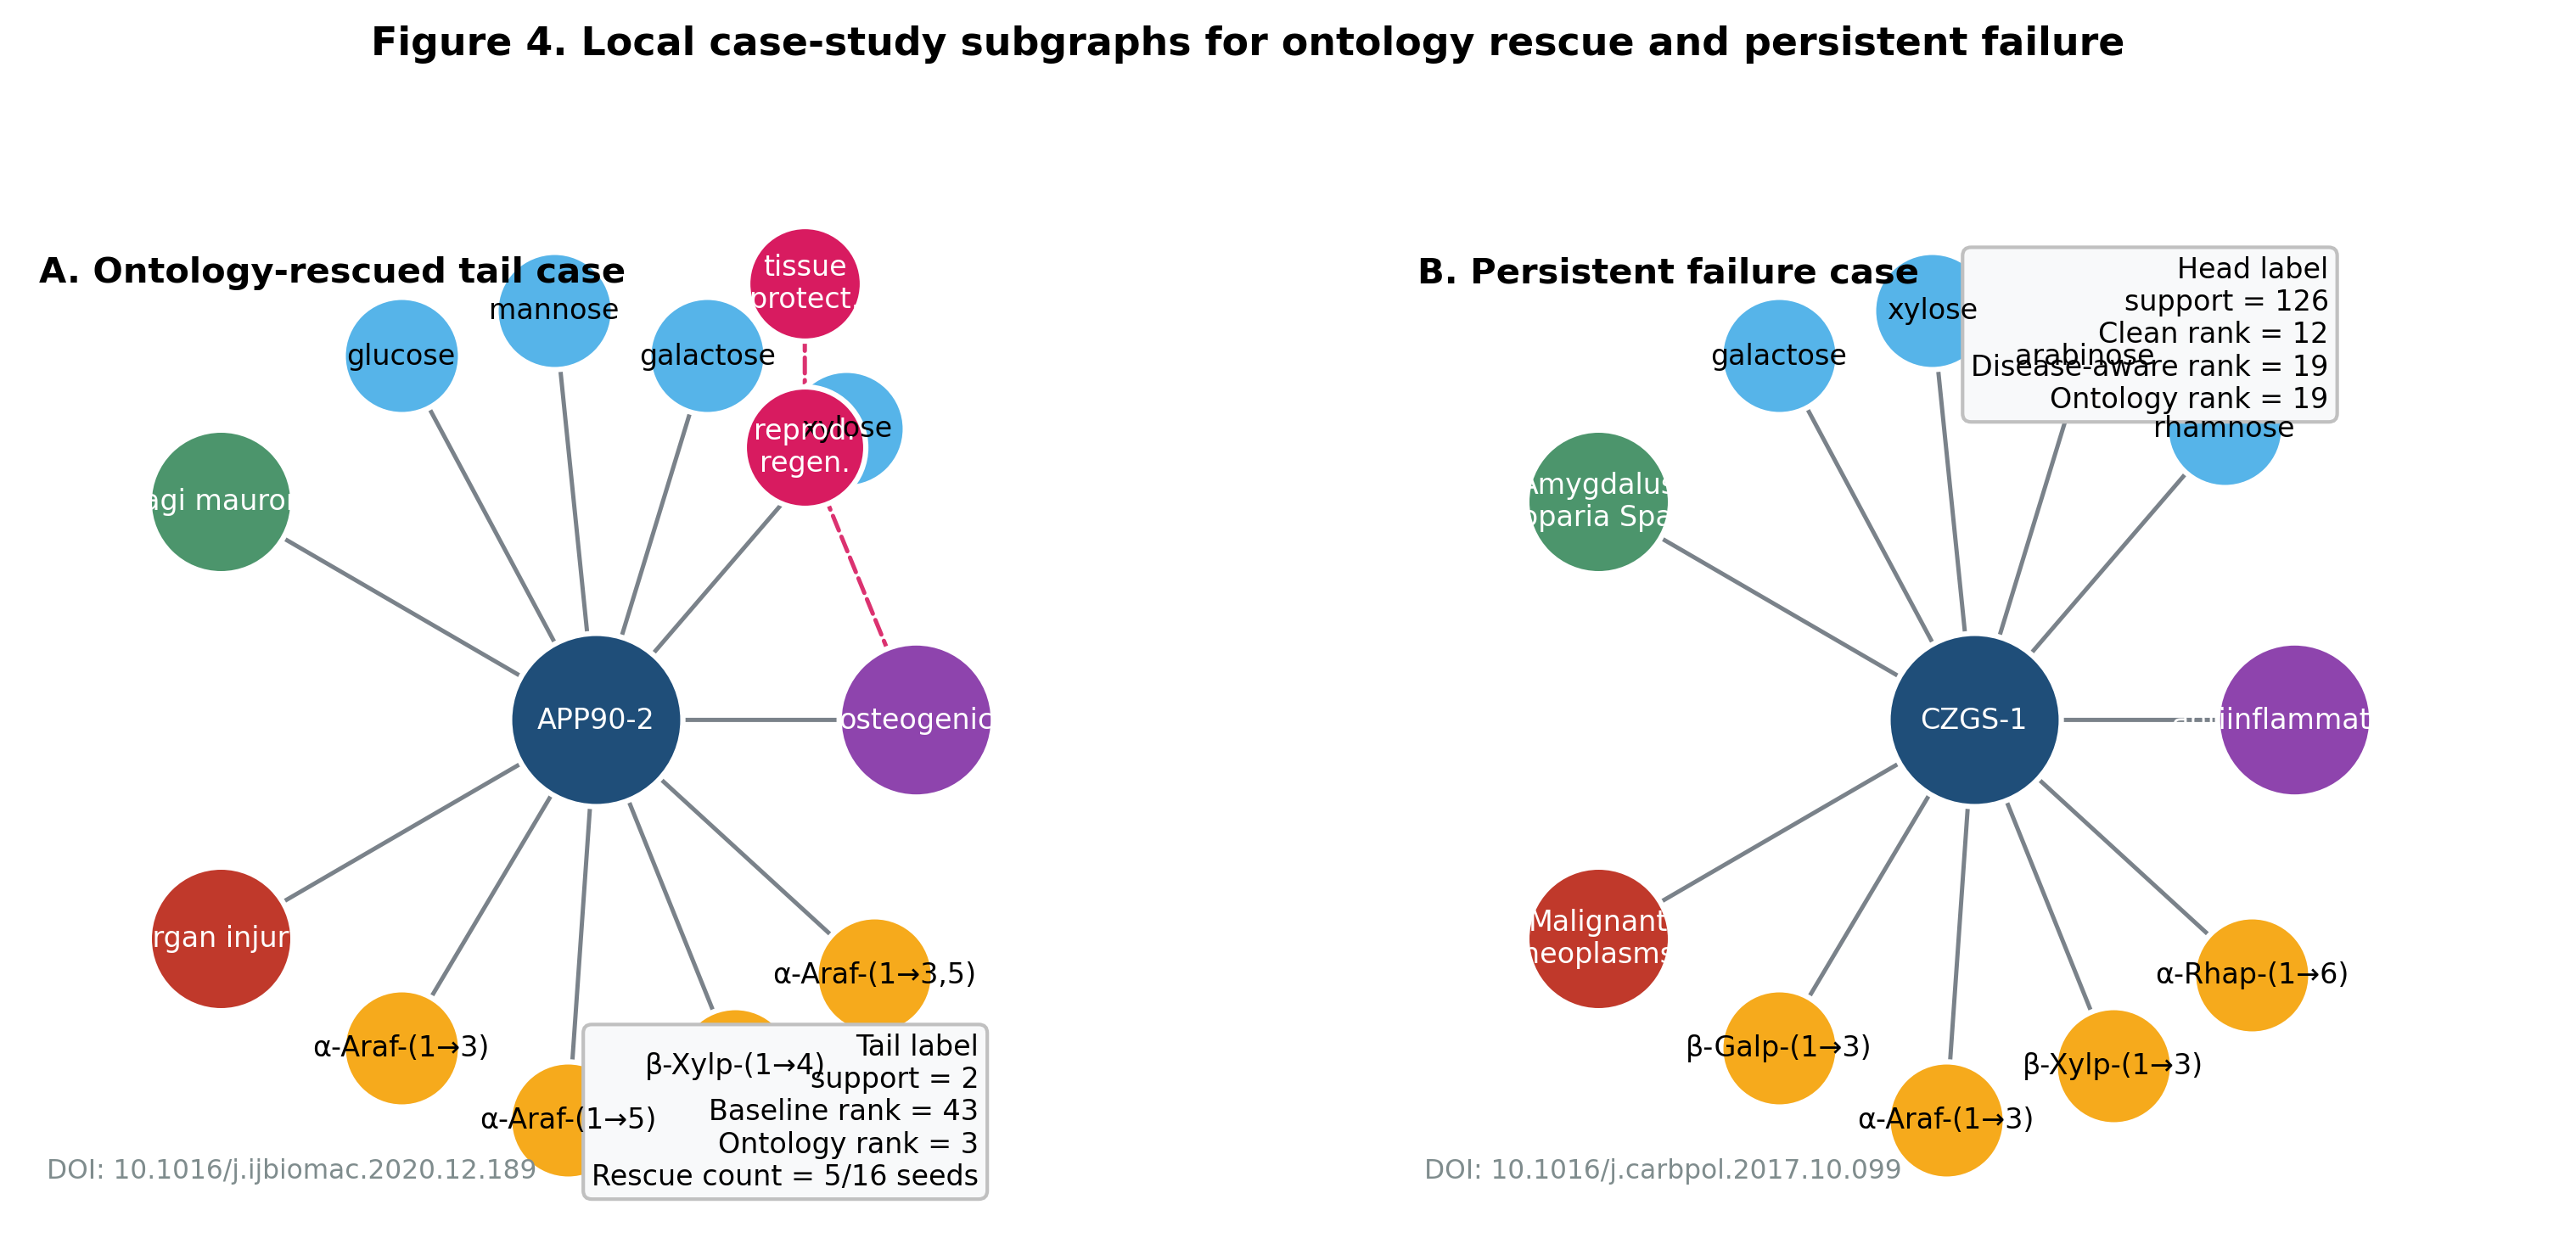
\includegraphics[width=0.96\textwidth]{../../paper/figures/figure4_case_subgraphs.png}
\caption{Biology-facing local case-study subgraphs. Panel A shows the ontology-rescued tail case \texttt{APP90-2} with held-out \texttt{osteogenic}, where confidence-gated parent/child propagation moves the label from filtered rank 43 to rank 3 through a narrow ontology path rather than a global family bonus. Panel B shows the persistent failure case \texttt{CZGS-1} with held-out \texttt{antiinflammatory}, where rich local evidence is present but the label remains at rank 12 in the clean setting and rank 19 in both the disease-aware baseline and ontology-enhanced setting. Together, the two panels illustrate both the promise and the boundary of ontology-aware retrieval on the current KG.}
\label{fig:case-subgraphs}
\end{figure*}

\subsection{Limitations}
\label{sec:limitations}

This paper should be read within a deliberately bounded scope. First, the clean and disease-aware settings answer different questions. The clean setting tests whether the graph itself contains useful structure-function signal, whereas the disease-aware setting estimates a practical upper bound when auxiliary semantics are available. Because disease is tightly coupled to the target functions, the disease-aware results should not be interpreted as a pure structure-only mechanism. The ontology claim is correspondingly narrow: the paired multi-seed analysis is the main stability evidence, while the tuned split is included only as an interpretable single operating point.

Second, the current function hierarchy is intentionally modest. It is sufficient to test whether ontology can help the tail, but it is not a comprehensive biological ontology of polysaccharide function. The parent/child propagation result should therefore be interpreted as proof of mechanism, not as the final possible ontology result.

Third, the graph remains structurally incomplete in several ways. Richer motif-level representations, external glycan ontologies, and more expressive provenance-aware evidence typing are not yet integrated. These missing components may matter for both cleaner biological interpretation and stronger end-to-end graph learning. The present manuscript therefore supports a constrained claim: the current graph is already useful for interpretable retrieval, and selective ontology propagation provides a stable tail-sensitive gain on top of that retrieval stack. It does not yet show that the current ontology formulation is biologically comprehensive or that current GNN baselines are competitive once stronger structure-aware evidence is introduced.

\section{Supplementary Data}
\label{sec:artifact-availability}

Supplementary Data include the normalized KG export, benchmark split definitions, the task-specific parent/child function hierarchy, paired edge-level stability records, the standalone supplementary PDF, case-study candidate tables, and the scripts used for graph construction, PyG export, retrieval, shallow baselines, GNN ablations, and figure generation. These assets will be released together with the public repository and database landing page at submission time.

\begin{table*}[t]
\centering
\caption{Paired stability and significance analysis for the ontology-enhanced variant. Reported values summarize 16 paired seeds and 16,000 masked edges. Unlike Table~\ref{tab:retrieval-results}, this table reports pooled paired-seed statistics rather than the representative tuned split. The ontology variant remains nearly unchanged in global effect size for aggregate Hits@3, while providing a statistically supported tail-sensitive gain. The filtered MRR difference is statistically detectable under paired testing, but its magnitude is practically negligible relative to the tail gain.}
\label{tab:stability}
\small
\begin{tabularx}{\textwidth}{>{\raggedright\arraybackslash}p{2.4cm}>{\centering\arraybackslash}p{1.15cm}>{\centering\arraybackslash}p{1.15cm}>{\centering\arraybackslash}p{1.25cm}>{\centering\arraybackslash}p{1.8cm}>{\raggedright\arraybackslash}X}
\toprule
Metric & Base. & Ont. & Delta & 95\% CI for delta & Statistical test / note \\
\midrule
Filtered MRR & 0.8430 & 0.8427 & -0.0003 & [-0.0004, -0.0001] & permutation, p = 0.0015; effect size negligible \\
Filtered Hits@3 & 0.9088 & 0.9085 & -0.0003 & [-0.0008, 0.0001] & McNemar two-sided, p = 0.3018 \\
Filtered Hits@5 & 0.9366 & 0.9366 & 0.0000 & [-0.0007, 0.0007] & permutation, p = 1.0000 \\
Tail micro filtered Hits@3 & 0.0552 & 0.1021 & \gain{+0.0469} & [0.0101, 0.1010] & McNemar one-sided, p = 0.03125 \\
Tail filtered MRR delta & - & - & \gain{+0.0395} & [0.0233, 0.0568] & permutation, p = 0.0002499 \\
\bottomrule
\end{tabularx}
\normalsize
\end{table*}

\section{Funding}
Insert funding information here.

\section{Acknowledgements}
Insert acknowledgements here.

\section{Conclusion}
\label{sec:conclusion}

We presented a DoLPHiN-derived heterogeneous polysaccharide knowledge graph and used it to study masked function retrieval as the primary benchmark together with clean function-prediction diagnostics and ontology-enhanced tail recovery. The central conclusion is not that a new model uniformly dominates prior baselines, but that the current KG already supports useful interpretable retrieval and a controlled benchmark for understanding what kinds of graph evidence matter. On this resource, the strongest clean model is an explicit shallow feature classifier rather than a hetero GNN, and full message passing is nearly indistinguishable from no-message ablations under the present graph representation. Disease-aware retrieval defines a strong upper-bound regime rather than the primary clean claim. Within that regime, confidence-gated parent/child ontology propagation yields a reproducible, proof-of-principle tail-sensitive improvement without changing the overall ranking profile in a practically meaningful way. Taken together, these results position the current graph as a useful benchmark and retrieval substrate for polysaccharide function studies, while also clarifying why current hetero GNN baselines underperform and where future representation work should focus.

\bibliographystyle{unsrt}
\bibliography{references}

\end{document}
